\title{State Machine Design}
\begin{document}
\section{Design Procedure}
\begin{frame}{Design types}
  Like all circuit design, state machine design usually starts with an English language description of the requirements. \\
  \begin{block}{Design Procedure}
    We can break state machine design down into two procedures:
    \begin{itemize}
      \item State table based design
      \item State diagram based design
    \end{itemize}
  \end{block}
\end{frame}

\subsection{State Table Design Procedure}

\begin{frame}{State table design procedure}
  This procedure is almost the opposite of the analysis procedure.
  \begin{enumerate}
    \item Construct a state/output table to describe the requirements.
    \item Assign state variables.
    \item Create a transition table.
    \item Construct the excitation table.
    \item Derive the excitation equations and output equations.
  \end{enumerate}
\end{frame}

\subsection{State Diagram Design Procedure}

\begin{frame}{State diagram design procedure}
    In many cases, it is not trivial to immediate create a state/output table listing all of the required states.
  \begin{enumerate}
    \item Start by drawing a state diagram.
    \item Run through each possible input combination and state transition based on real usage scenarios.
    \item Modify that original state diagram.
    \item Once the state diagram seems to be complete, construct the state/output table and continue with the state table based design procedure.
  \end{enumerate}
\end{frame}

\section{State Table Design Example}

\begin{frame}{Problem definition}
  Design a clocked synchronous state machine with two inputs, A and B, and a single output Z that is 1 if:
  \begin{itemize}
    \item A had the same value at each of the two previous clock ticks, or
    \item B has been 1 since the last time that the first condition was true.
  \end{itemize}
  Otherwise the output should be zero.
\end{frame}

Note that in this state machine, the state is not as important as the output.

\begin{frame}{State/output table}
  Step 1: Construct the state/output table.
\end{frame}

\begin{tabular}{lc|cccc|c}
  Meaning & S & 00 & 01 & 11 & 10 & Z \\
  \hline
  Initial state & INIT & A0 & A0 & A1 & A1 & 0 \\
  Got a 0 on A & A0 & A0OUT & A0OUT & A1 & A1 & 0 \\
  Got a 1 on A & A1 & A0 & A0 & A1OUT & A1OUT & 0 \\
  Two equal, A=0 last & AOOUT & A0OUT & A0OUT & A1OUT & A1 & 1 \\
  Two equal, A=1 last & A1OUT & A0 & A0OUT & A1OUT & A1OUT & 1 \\
\end{tabular}

\begin{frame}{Assign state variables}
  Step 2: Assign state variables. \\
  Choose the type and number of flip-flops to implement the state memory.
  \begin{itemize}
    \item Choose an initial state that is easy to preset.
    \item Minimize the number of state variables that change on each transition.
    \item Give each state variable a well-defined means with respect the to inputs or the outputs of the state machine.
    \item Assign one state variable per state.
  \end{itemize}
  The right decision may vary based on the requirements, and finding it is often a result of experience or trial and error.
\end{frame}

Use 3 D flip-flops. \\

\begin{tabular}{c|cccc}
  S & Q1-Q3 & Q1-Q3 & Q1-Q3 & Q1-Q3 \\
  \hline
  INIT  & 000 & 000 & 00001 & 0000 \\
  A0    & 001 & 100 & 00010 & 0001 \\
  A1    & 010 & 101 & 00100 & 0010 \\
  AOOUT & 011 & 110 & 01000 & 0100 \\
  A1OUT & 100 & 111 & 10000 & 1000 \\
\end{tabular}

\begin{frame}{Transition table}
  Step 3: Create the transition table.
\end{frame}

\begin{tabular}{c|cccc}
  Q1Q2Q3 & 00 & 01 & 11 & 10 \\
  \hline
  000 & 100 & 100 & 101 & 101 \\
  100 & 110 & 110 & 101 & 101 \\
  101 & 100 & 100 & 111 & 111 \\
  110 & 110 & 110 & 111 & 101 \\
  111 & 100 & 110 & 111 & 111 \\
\end{tabular}

\begin{frame}{Excitation table}
  Step 4: Construct the excitation table.
\end{frame}

Note $Q*=D$ for the D flip-flop.

\begin{tabular}{c|cccc|c}
  Q1Q2Q3 & 00 & 01 & 11 & 10 & Z\\
  \hline
  000 & 100 & 100 & 101 & 101 & 0\\
  100 & 110 & 110 & 101 & 101 & 0\\
  101 & 100 & 100 & 111 & 111 & 0\\
  110 & 110 & 110 & 111 & 101 & 1\\
  111 & 100 & 110 & 111 & 111 & 1\\
\end{tabular}

\begin{frame}{Excitation and output equations}
  Step 5: Derive the excitation and output logic equations.
  \begin{itemize}
    \item Create Karnaugh maps based on the excitation table.
    \item Note that unused states should be represented by zeros in the Karnaugh map.
    \item Do five variable Karnaugh maps using two four variable Karnuagh maps.
  \end{itemize}
\end{frame}

\begin{frame}{Karnaugh map for D1}
  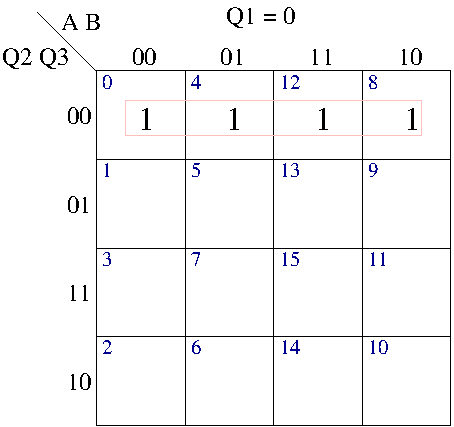
\includegraphics[scale=0.7]{D1Q1is0KMap}
  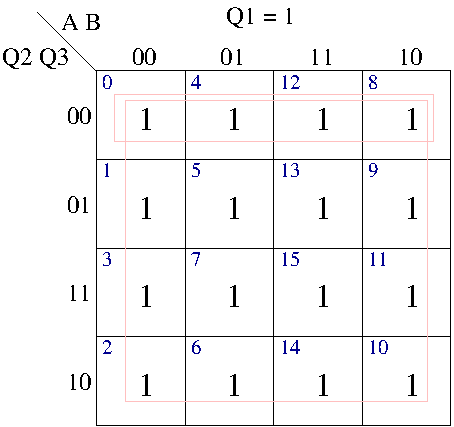
\includegraphics[scale=0.7]{D1Q1is1KMap}
\end{frame}

$$D1 = Q1 + Q2' \cdot Q3'$$

\begin{frame}{Karnaugh map for D2}
  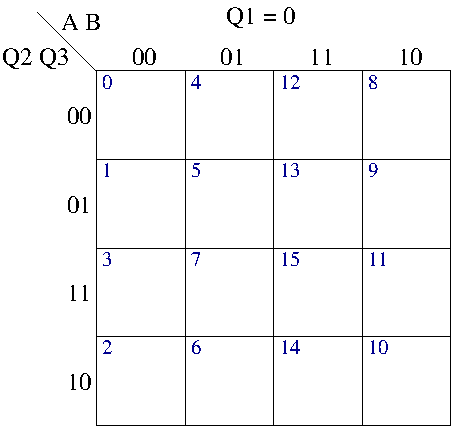
\includegraphics[scale=0.7]{D2Q1is0KMap}
  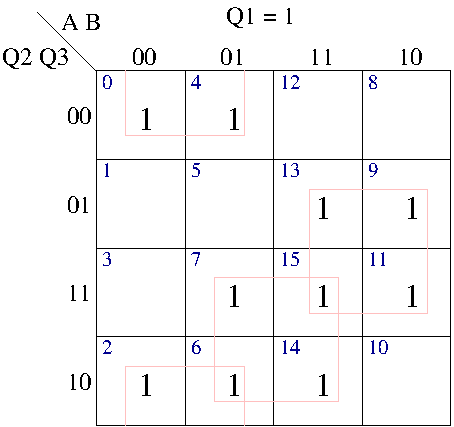
\includegraphics[scale=0.7]{D2Q1is1KMap}
\end{frame}

$$D2 = Q1 \cdot Q3' \cdot A' + Q1 \cdot Q3 \cdot A + Q1 \cdot Q2 \cdot B$$

\begin{frame}{Karnaugh map for D3}
  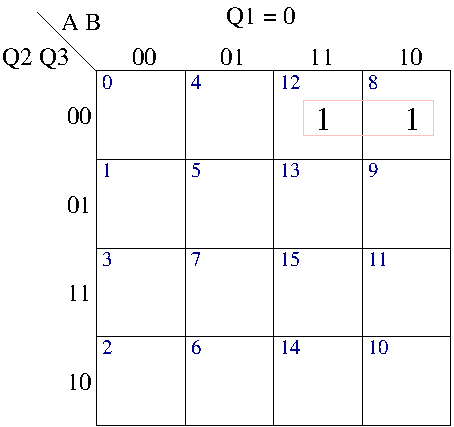
\includegraphics[scale=0.7]{D3Q1is0KMap}
  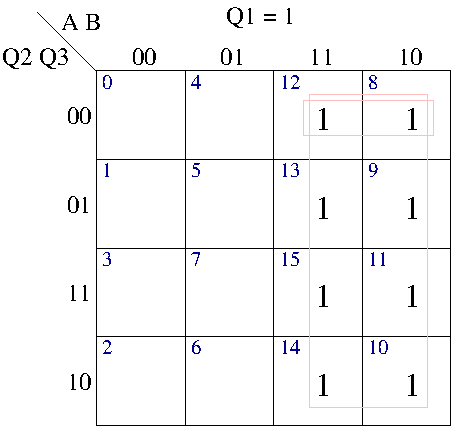
\includegraphics[scale=0.7]{D3Q1is1KMap}
\end{frame}

$$D3 = Q1 \cdot A + Q2' \cdot Q3' \cdot A$$

\begin{frame}{Output equation}
  In this case, we can write a sum of minterms logic function and simplify it by hand.
  $$Z = Q1 \cdot Q2 \cdot Q3' + Q1 \cdot Q2 \cdot Q3 = Q1 \cdot Q2$$
\end{frame}

\section{State Diagram Design Example}

\begin{frame}{GPS limit warning system}
  A railroad maintenance vehicle must remain within specific limits to maintain safety.
  \begin{itemize}
    \item We know whether the vehicle is on or off the track.
    \item We know whether the vehicle is in or out of its limits (GPS position).
    \item We know the velocity (speed and direction) of the vehicle.
  \end{itemize}
  Create a state diagram that transitions on each GPS update and outputs a warning if the worker should begin braking and an error if the worker has exceeded the limits.
\end{frame}

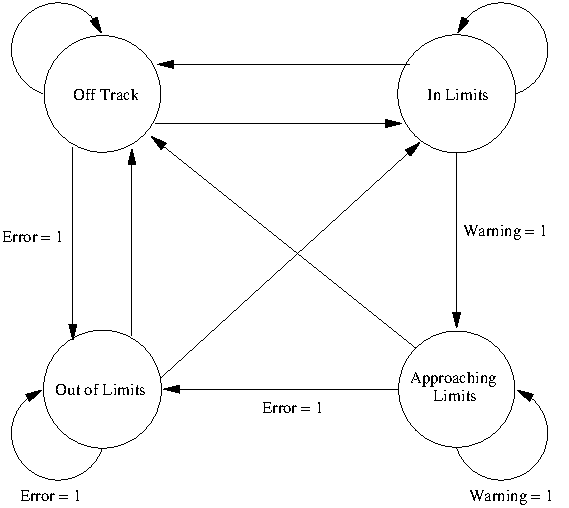
\includegraphics{GPSLimitWarningStateDiagram}

\end{document}
